\section{Datenbeschaffung}

\frame{
  \frametitle{Überblick}
  \tableofcontents[currentsection,hidesubsections,firstsection=5]
}

    %---------------------------------------------------------------------

\section{Heterogenität und Datenfehler}

\frame{
  \frametitle{Überblick}
  \tableofcontents[currentsection,hidesubsections,firstsection=5]
}


\begin{frame}
    \frametitle{Data-Science-Prozess Revisited}
    
    \begin{center}
    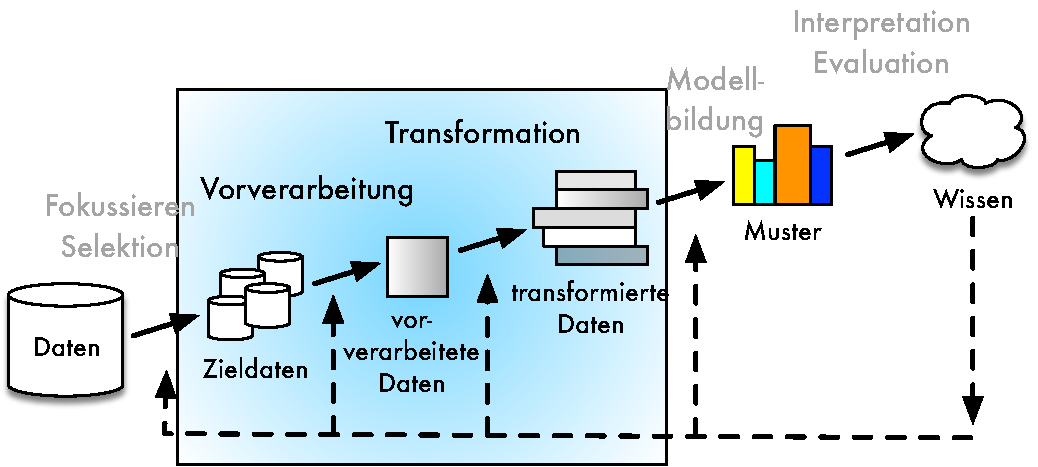
\includegraphics[scale=.6]{fig4/kdd-prozess.pdf}
    \end{center}
    
    \begin{itemize}
    \item notwendig wegen \hl{Heterogenität} durch Integration
      verschiedener Quellen und möglichen \hl{Datenfehlern}
    \end{itemize}
    
    \end{frame}
    
    %---------------------------------------------------------------------
    
    \begin{frame}
    \frametitle{Motivation: Heterogenität}
    
    \begin{itemize}
    \item \hl{verschiedene Datenmodelle}
    \begin{itemize}
    % \item bedingt durch autonome Entscheidung �ber Anschaffung von
    %   Systemen in den Unternehmensbereichen 
    \item verschiedene und verschieden mächtige Modellierungskonstrukte,
      d.h. Anwendungssemantik in unterschiedlichem Ausmaß erfassbar 
    \item Abbildung zwischen Datenmodellen nicht eindeutig
    \end{itemize}
    \item \hl{unterschiedliche Modellierungen für gleiche Sachverhalte der
        Realwelt}  
    \begin{itemize}
    \item bedingt durch Entwurfautonomie
    \item selbst im gleichen Datenmodell verschiedene Modellierungen
      möglich, z.B. durch unterschiedliche Modellierungsperspektiven 
    \end{itemize}
    \end{itemize}
    
    \end{frame}
    
    %---------------------------------------------------------------------
    
    \begin{frame}
    \frametitle{Motivation: Heterogenität /2}
    
    \begin{itemize}
    \item \hl{unterschiedliche Repräsentation der Daten}
    \begin{itemize}
    \item unterschiedliche Datentypen möglich
    \item unterschiedliche Umfang der unterstützten Datentypen
    \item unterschiedliche interne Darstellung der Daten
    \item auch unterschiedliche "`Werte"' eines Datentyps zur
      Repräsentation derselben Information 
    \end{itemize}
    \end{itemize}
    
    \end{frame}
    
    %---------------------------------------------------------------------
    
    
    \begin{frame}
    \frametitle{Datenfehler}
    
    \begin{overlayarea}{\textwidth}{5cm}
    
    \begin{center}
    \only<1| handout:0>{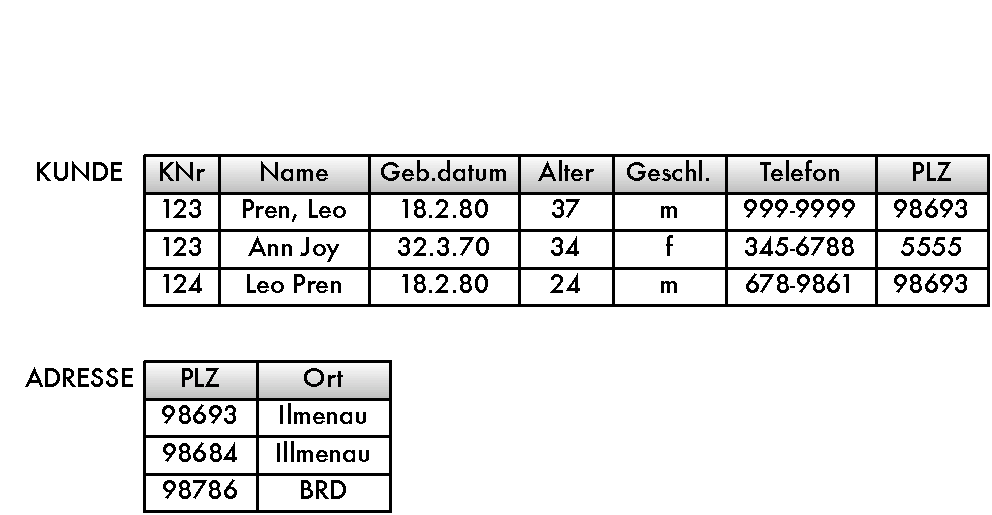
\includegraphics[scale=.6]{fig4/datenfehler-1.pdf}}
    \only<2>{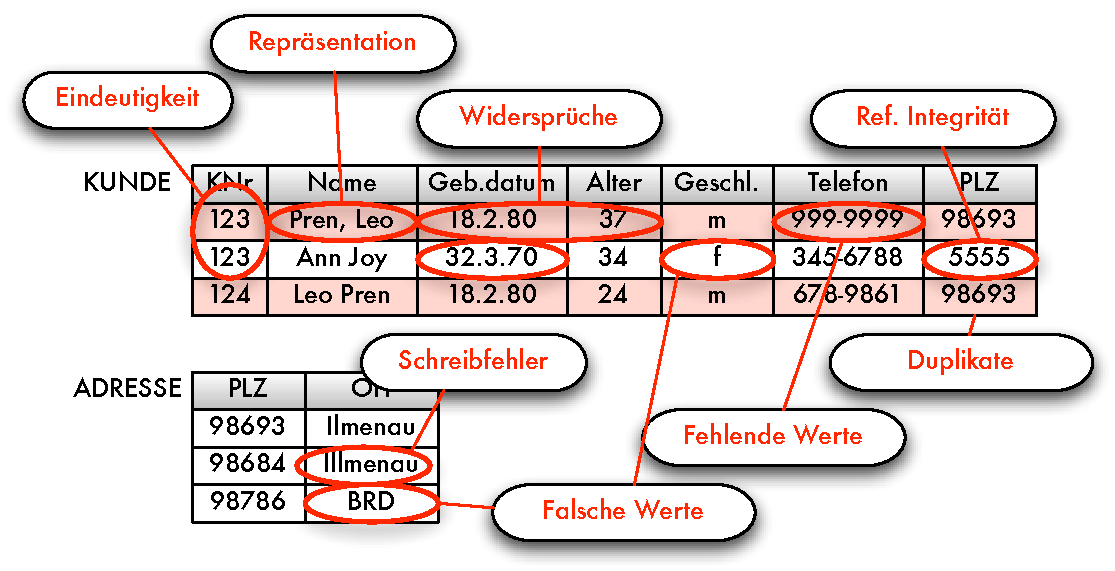
\includegraphics[scale=.6]{fig4/datenfehler-2.pdf}}
    \end{center}
    
    \end{overlayarea}
    \end{frame}
    
    %---------------------------------------------------------------------
    
    \begin{frame}
    \frametitle{Vermeidung von Datenfehlern}
    
    \begin{tabular}{ll}
    \textbf{Vermeidung von}	& \textbf{durch} \\
    \hline
    falschen Datentypen &	Datentypdefinition, \\
    & \op{domain}-Constraints \\
    falschen Werten &	\op{check} \\
    fehlenden Werten &	\op{not null} \\
    ungültigen Referenzen &	\op{foreign key} \\
    Duplikaten &	\op{unique}, \op{primary key} \\
    Inkonsistenzen & Transaktionen \\
    veralteten Daten & Replikation, materialisierte Sichten \\
    \end{tabular}
    \end{frame}
    
    %---------------------------------------------------------------------
    
    \begin{frame}
    \frametitle{Warum dennoch Datenfehler?}
    
    \begin{itemize}
    \item Fehlen von Metadaten, Integritätsbedingungen, \dots
    \item "`fremde"' Daten
    \item Daten aus "`Nicht-DB"'-Quellen
    \item Eingabefehler, Unkenntnis, \dots
    \item Multi-Source-Probleme, Heterogenitäten
    \end{itemize}
    
    \end{frame}
    
    %---------------------------------------------------------------------
    
    \begin{frame}
    \frametitle{Phasen der Datenaufbereitung}
    
    \begin{center}
    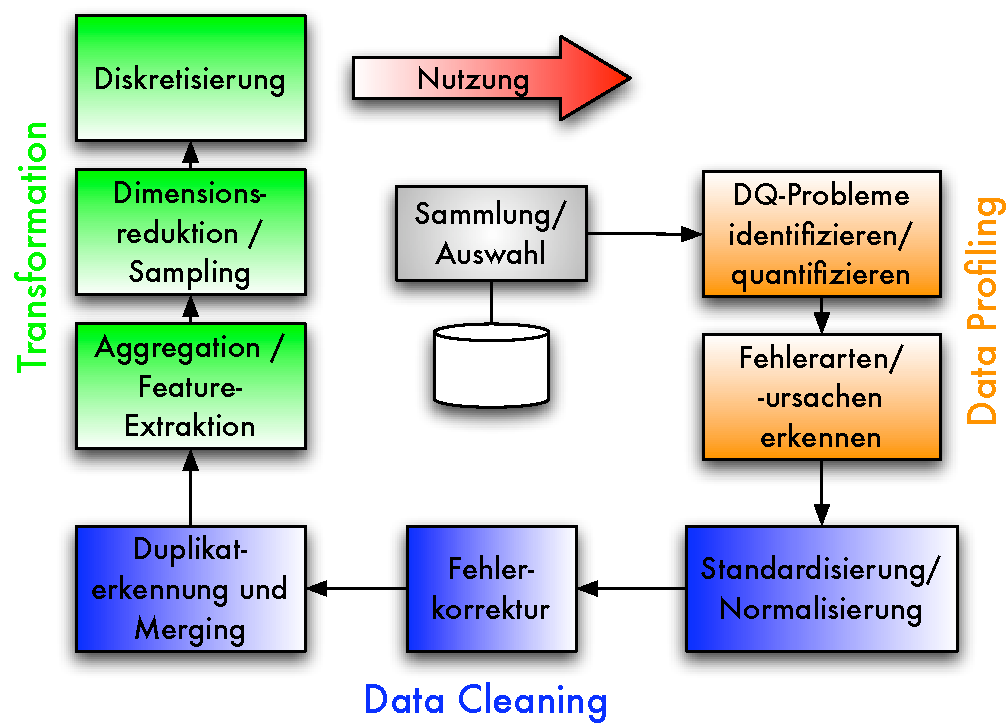
\includegraphics[scale=.5]{fig4/data-preparation.pdf}
    \end{center}
    
    \end{frame}
    
    %---------------------------------------------------------------------
    
    \begin{frame}
    \frametitle{Aufgaben}
    
    \begin{itemize}
    \item Profiling
    \item Homogenisierung und Normalisierung
    \item Behandlung fehlender Daten / Werte
    \item Ausreißererkennung
    \item Record Linkage / Matching, Konfliktbehandlung
    \item Datenaufbereitung: Diskretisierung, Sampling, .... 
    \end{itemize}
    \end{frame}
    
    %---------------------------------------------------------------------
    
    
    \section{Profiling}
    
    
    \frame{
      \frametitle{Überblick}
      \tableofcontents[currentsection,hidesubsections,firstsection=5]
    }
    
    %---------------------------------------------------------------------
    
    \begin{frame}
    \frametitle{Profiling}
    
    \begin{itemize}
    \item Analyse von Inhalt und Struktur einzelner Attribute
    \begin{itemize}
    \item Datentyp, Wertebereich, Verteilung und Varianz, Vorkommen von
      Nullwerten, Eindeutigkeit, Muster (z.B. dd/mm/yyyy) 
    \end{itemize}
    \item Analyse von Abhängigkeiten zwischen Attributen einer Relation
    \begin{itemize}
    \item "`unscharfe"' Schlüssel
    \item Funktionale Abhängigkeiten, potenzielle Primärschlüssel,
      "`unscharfe"' Abhängigkeiten 
    \item Notwendigkeit:
    \begin{itemize}
    \item Keine expliziten Integritätsbedingungen spezifiziert
    \item Jedoch in Daten in den meisten Fällen erfüllt
    \end{itemize}
    \end{itemize}
    \item Analyse von Überlappungen zwischen Attributen verschiedener Relationen
    \begin{itemize}
    \item Redundanzen, Fremdschlüsselbeziehungen
    \end{itemize}
    \end{itemize}
    
    \end{frame}
    
    %---------------------------------------------------------------------
    
    \begin{frame}
    \frametitle{Profiling /2}
    
    \begin{itemize}
    \item Fehlende bzw. falsche Werte
    \begin{itemize}
    \item Ermittelte vs. Erwartete Kardinalität (z.B. Anzahl von Filialen, Geschlecht von Kunden)
    \item Anzahl der Nullwerte, Minimum / Maximum, Varianz
    \end{itemize}
    \item Daten- bzw. Eingabefehler
    \begin{itemize}
    \item Sortierung und manuelle Prüfung
    \item Ähnlichkeitstest
    \end{itemize}
    \item Duplikate
    \begin{itemize}
    \item Tupelanzahl vs. Attributkardinalität
    \end{itemize}
    \end{itemize}
    
    
    \end{frame}
    
    %---------------------------------------------------------------------
    
    
    % \begin{frame}
    % \frametitle{Profiling mit SQL}
    
    % \begin{itemize}
    % \item SQL-Anfragen f�r einfache Profiling-Aufgaben
    % \begin{itemize}
    % \item Schema, Datentypen: Anfragen an Schemakatalog
    % \item Wertebereich
    % \hspace*{-1cm}\begin{sql}
    % \op{select min}(A), \op{max}(A), \op{count}(\op{distinct} A) \\
    % \op{from} Tabelle
    % \end{sql}
    % \item Datenfehler, Defaultwerte
    % \hspace*{-1cm}\begin{sql}
    % \op{select} Ort, \op{count}(*) \op{as} Anz\\
    % \op{from} Kunden \op{group by} Ort \op{order by} Anz
    % \end{sql}
    % \begin{itemize}
    % \item Aufsteigend: Eingabefehler, z.B. Illmenau: 1, Ilmenau: 50
    % \item Absteigend: undokumentierte Default-Werte, z.B. AAA: 80
    % \end{itemize}
    % \end{itemize}
    % \end{itemize}
    % \end{frame}
    
    %---------------------------------------------------------------------
    
    
    \section{Datenbereinigung}
    
    
    \frame{
      \frametitle{Überblick}
      \tableofcontents[currentsection,hidesubsections,firstsection=5]
    }
    
    
    \begin{frame}
    \frametitle{Data Cleaning}
    
    \begin{itemize}
    \item Erkennen \& Beseitigen von Inkonsistenzen, Widersprüchen und
      Fehlern in Daten mit dem Ziel der Qualitätsverbesserung  
    \item Auch Cleansing oder Scrubbing
    \item Bis zu 80\% des Aufwandes in DW-Projekten
    \item Cleaning im DW: Teil des ETL-Prozesses
    \end{itemize}
    
    \end{frame}
    
    %---------------------------------------------------------------------
    
    \begin{frame}
    \frametitle{Normalisierung und Standardisierung}
    
    \begin{itemize}
    \item Datentypkonvertierung: varchar $\rightarrow$ int
    \item Normalisierung: Abbildung in einheitliches Format
    \begin{itemize}
    \item Datum: 03/01/15 $\rightarrow$ 1. März 2015
    \item Währung: \$ $\rightarrow$ \euro
    \item Zeichenketten in Großbuchstaben
    \end{itemize}
    \item Zerlegung in Token: ``Metallica - ...And Justice for All'' $\rightarrow$ ``Metallica'', ``...And Justice for All''
    \item Diskretisierung numerischer Werte (Aufteilung von Wertebereichen in Intervalle, z.B. Altersgruppen)
    \item Domänenspezifische Transformationen
    \begin{itemize}
    \item Codd, Edgar Frank $\rightarrow$ Edgar Frank Codd
    \item Str. $\rightarrow$ Straße
    \item Adressen über Adressdatenbanken
    \item Branchenspezifische Produktbezeichnungen
    \end{itemize}
    \end{itemize}
    
    \end{frame}
    
    %---------------------------------------------------------------------
    
    \begin{frame}
    \frametitle{Normalisierung numerischer Daten}
    
    \begin{itemize}
    \item Skalierung der Werte $v$ eines Attributs $A$ mit $[min_A,max_A]$
      in vorgegebenen Bereich $[min_{new},max_{new}]$, z.B. $[0, 1]$
    % \item notwendig u.a. f�r distanzbasierte Verfahren
    % \item Techniken
    \begin{itemize}
    \item Min-Max-Normalisierung
    $$
    v' = \frac{v - min_A}{max_A - min_A}(max_{new} - min_{new}) +
    min_{new}
    $$
    \item Z-Score-Normalisierung: basierend auf Mittelwert und
      Standardabweichung
    $$
    v' = \frac{v - \mu}{\sigma}
    $$
    \begin{itemize}
    \item speziell wenn $min_A$, $max_A$ nicht bekannt sind oder bei
      dominierenden Ausreißern
    \end{itemize}
    \item Dezimalskalierung: "`Verschieben"' des Dezimalpunktes
    $$
    v' = \frac{v}{10^i}\;\text{mit}\;i\;\text{ist kleinster ganzzahliger
      Wert, sodass}\;max(|v'|) < 1
    $$
    \end{itemize}
    
    \end{itemize}
    
    \end{frame}
    
    %---------------------------------------------------------------------
    
    \begin{frame}
    \frametitle{Fehlende Werte}
    
    \begin{itemize}
    \item Fehlen von Daten auf unterschiedlichen Ebenen
    \begin{itemize}
    \item Instanzebene: Werte, Datensätze, Teilrelationen, ...
    \item Schemaebene: Attribute, ...
    \end{itemize}
    \item Problem speziell auf Instanzebene:
    \begin{itemize}
    \item Behandlung von Nullwerten: Unterscheidung fehlender Wert, Defaultwert oder Dummywert? 
    \item "`Abschneiden"' von Werten
    \end{itemize}
    \item Verzerrungen von Erwartungswerten, Fehler durch Nullwerte
    \end{itemize}
    
    \end{frame}
    
    %---------------------------------------------------------------------
    
    \begin{frame}
    \frametitle{Fehlende Werte: Erkennung}
    
    \begin{itemize}
    \item Einfache Analysen: 
    \begin{itemize}
    \item Anzahl der Nullwerte, Duplikate, Mittelwerte, Häufigkeiten
    \item Vergleich mit Erwartungswerten
    \item Für DW-Daten auch auf verschiedenen Aggregationsebenen
    \end{itemize}
    \item Analyse der "`Ordnung"' der Datensätze
    \begin{itemize}
    \item Keine Verkaufszahlen vom 1.3.-4.3.?
    \item Keine Produkte im Preissegment > 20 \euro?
    \end{itemize}
    \item "`Verstümmelte"' Daten, z.B. durch Abschneiden von Werten
    \begin{itemize}
    \item Einkäufe unter 1 \euro\ nicht berücksichtigt
    \item Einkäufe über 100 \euro\ als 100 \euro\ behandelt
    \end{itemize}
    \item Erkennung
    \begin{itemize}
    \item Hinweise durch Analyse der Datenverteilung
    \item Meist jedoch Domänenwissen notwendig 
    \end{itemize}
    \end{itemize}
    
    \end{frame}
    
    %---------------------------------------------------------------------
    
    
    \begin{frame}
    \frametitle{Fehlende Werte: Behandlung}
    
    \begin{itemize}
    \item "`unbiased estimators"'
    \begin{itemize}
    \item Wertschätzung ohne Änderung der Charakteristika der
      existierenden Daten (Mittelwert, Standardabweichung, \dots) 
    \item Beispiel: 1, 2, 3, \_, 5
    \begin{itemize}
    \item Mittelwert erhalten $\rightarrow$ 2.75
    \item Standardabweichung erhalten $\rightarrow$ 4.659
    \end{itemize}
    \end{itemize}
    \item Ausnutzung von Attributbeziehungen
    \begin{itemize}
    \item Bsp.: Hausgröße $\rightarrow$ Einkommen
    \end{itemize}
    \item Statistik-Techniken
    \begin{itemize}
    \item Lineare Regression: Einkommen = c $\cdot$ Hausgröße
    \item Techniken für nichtlineare Zusammenhänge: Neuronale Netze, \dots
    \end{itemize}
    \end{itemize}
    
    \end{frame}
    
    %---------------------------------------------------------------------
    
    \begin{frame}
    \frametitle{Profiling mit Pandas}
    
    \begin{itemize}
    \item Überblick zu den Daten
    \end{itemize}
    
    \begin{python}
    \prompt{In [10]:} kreise.describe()
    \end{python}
    
    \begin{itemize}
    \item Verteilung der Attributwerte
    \end{itemize}
    
    \begin{python}
    \prompt{In [11]:} kreise.hist(bins=20, figsize=(30,25))
    \end{python}
    
    \begin{itemize}
    \item Plotten der Korrelationen
    \end{itemize}
    
    \end{frame}
    
    %---------------------------------------------------------------------
    
    \begin{frame}
    \frametitle{Ausreißererkennung}
    
    \begin{itemize}
    \item Ausreißer: Wert der nicht in eine erwartete Messreihe passt
    \item Aspekte:
    \begin{itemize}
    \item Erkennung: Verteilung, "`Geometrie"', Zeitreihe
    \item Interpretation: Mess- bzw. Datenfehler oder echtes Ereignis
    \end{itemize}
    \begin{center}
    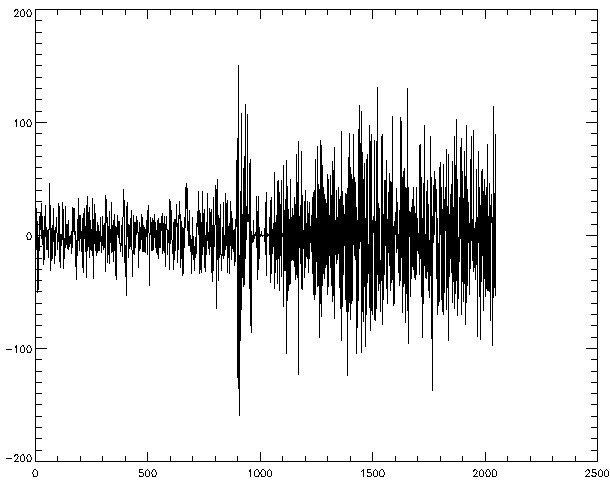
\includegraphics[width=4cm]{fig4/noise2.png}\quad
    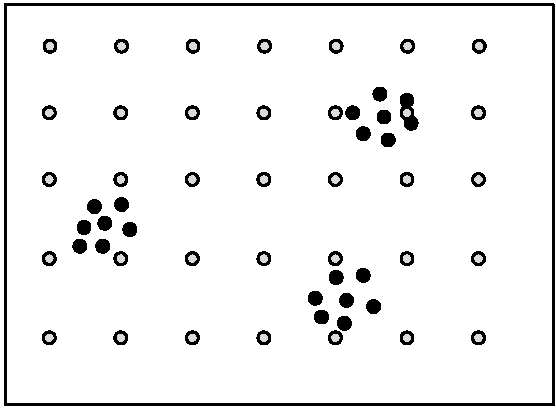
\includegraphics[width=4cm]{fig4/noise1.pdf}
    \end{center}
    \end{itemize}
    
    \end{frame}
    
    %---------------------------------------------------------------------
    
    \begin{frame}
    \frametitle{Ausreißererkennung /2: Erkennung }
    
    \begin{itemize}
    \item Modellbasiert: Ableitung einer Beziehung von Attributen
        \begin{itemize}
        \item lineare Regression
        \item Regeln: WENN Alter $<$ 16 DANN Führerschein IS NULL
        \end{itemize}
    \item Verteilungs- bzw. statistikbasiert: 
        \begin{itemize}
        \item z.B. Verwendung von Boxplots / Box-Whisker-Plots (außerhalb des Whiskers $\rightarrow$ Ausreißer)
        \end{itemize}
    
    \item Geometrisch und distanzbasiert:
    \begin{itemize}
    \item Peeling: "`Schichten"' im Datenraum mit wachsender Tiefe
    \begin{itemize}
    \item äußere Schichten enthalten Ausreißer
    \item Nicht praktikabel für höhere Dimensionsanzahl
    \end{itemize}
    \item Distanzbasiert: Abstand zwischen Datenpunkten (metrische
      Distanzfunktion) 
    \begin{itemize}
    \item Für Anwendungen ohne Standardverteilung
    \item Bei größerer Dimensionsanzahl
    \end{itemize}
    \end{itemize}
    \end{itemize}
    
    
    \end{frame}
    
    %---------------------------------------------------------------------
    
    \begin{frame}
    \frametitle{Distanzbasierte Ausreißer (\emph{DB})}
    
    \begin{itemize}
    \item Objekt $o$ aus Datenmenge $T$ ist Ausreißer $DB(p,D)$, wenn
      mindestens ein Anteil $p$ von $T$ weiter als $D$ von $o$ entfernt
      ist [Knorr Ng 1998] 
    \begin{columns}[c]
    \begin{column}{5cm}
    \begin{itemize}
    \item Ausreißer: "`Objekte, die nicht genug Nachbarn besitzen"'
    \item $p$ als Parameter zur Anpassung, falls Cluster von Ausreißern
    \item Bsp. Standardnormalverteilung: $DB(0.998, 0.13\sigma)$, $d \approx 3$
    \end{itemize}
    \end{column}
    \begin{column}{5cm}
    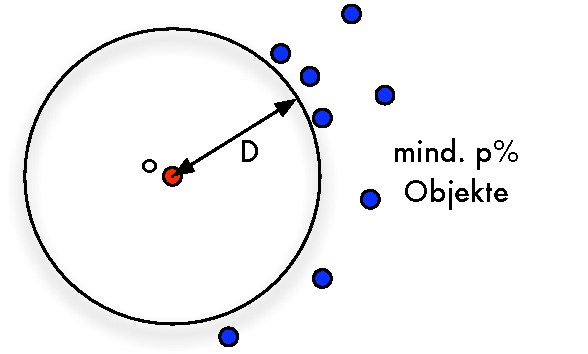
\includegraphics[scale=.6]{fig4/distance-outlier.pdf}
    \end{column}
    \end{columns}
    
    \end{itemize}
    
    
    \end{frame}
    
    
    %---------------------------------------------------------------------
    
    \begin{frame}
    \frametitle{Record Linkage}
    
    \begin{itemize}
    \item Identifikation von semantisch äquivalenten Datensätzen, d.h. die
      das gleiche Realwelt-Objekt repräsentieren
    \item auch: Object Identification, Duplicate Elimination, Merge/Purge
    \begin{itemize}
    \item Merge: Erkennen von Duplikaten
    \item Purge: Auswahl /Berechnung des "`besten"' Vertreters pro Klasse
    \end{itemize}
    \end{itemize}
    
    \begin{center}
    {\small\begin{tabular}{|c|l|l|}
    \hline
    \rowcolor{Gray} KundenNr & Name & Adresse \\
    \hline \hline
    3346 & Just Vorfan & Hafenstraße 12 \\
    3346 & Justin Forfun & Hafenstr. 12 \\
    \hline
    5252 & Lilo Pause & Kuhweg 42 \\
    5268 & Lisa Pause & Kuhweg 42 \\
    \hline
    $\perp$ & Ann Joy & Domplatz 2a \\
    $\perp$ & Anne Scheu & Domplatz 28 \\
    \hline
    \end{tabular}}
    \end{center}
    
    \end{frame}
    
    %---------------------------------------------------------------------
    \begin{frame}
    \frametitle{Record Linkage: Vergleiche}
    
    \begin{itemize}
    \item Typische Vergleichsregeln
    
    \hspace*{-1cm}\begin{sql}
    \op{if} ssn1=ssn2 \op{then} match \\
    \op{else} \op{if} name1=name2 \op{then} \\
    \1  \op{if} firstname1=firstname2 \op{then} \\
    \2    \op{if} adr1=adr2 \op{then} match \\
    \2    \op{else} unmatch \\
    \1  \op{else} \op{if} adr1=adr2 \op{then} match\_household \\
    \op{else} \op{if} adr1=adr2 \op{then} \\
     ...
    \end{sql}
    
    \item Naiver Ansatz: "`Jeder-gegen-jeden"'
    \begin{itemize}
    \item $O(n^2)$ Vergleiche
    \item Maximale Genauigkeit (je nach Regeln)
    \item Viel zu teuer
    \end{itemize}
    \end{itemize}
    
    \end{frame}
    
    %---------------------------------------------------------------------
    
    \begin{frame}
    \frametitle{Record Linkage: Prinzip}
    
    \begin{center}
    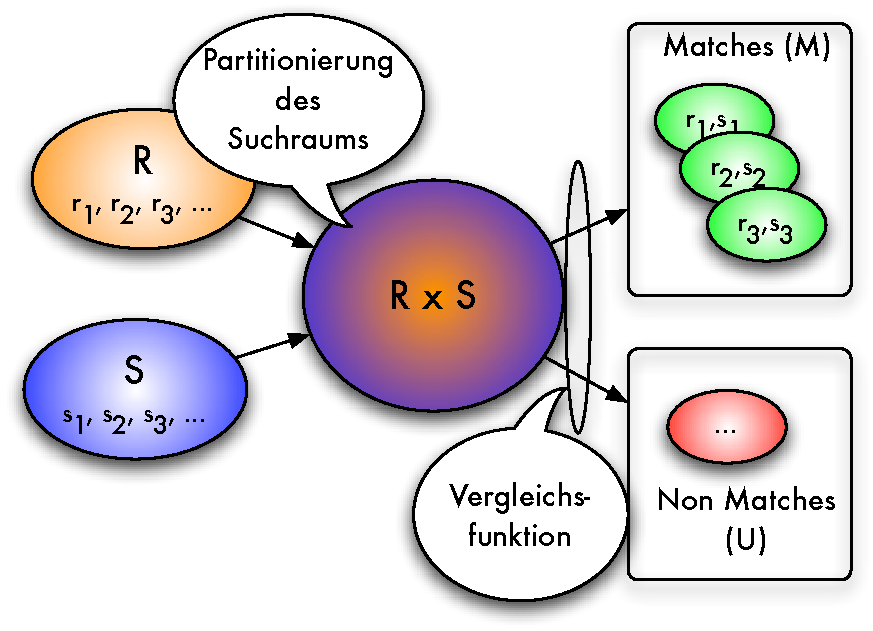
\includegraphics[scale=.6]{fig4/record-linkage.pdf}
    \end{center}
    
    \end{frame}
    
    %---------------------------------------------------------------------
    
    
    \begin{frame}
    \frametitle{Partitionierung}
    
    \begin{itemize}
    \item \hl{Blockung}
    \begin{itemize}
    \item Aufteilung des Suchraums in disjunkte Blöcke
    \item Duplikate nur innerhalb eines Blockes 
    \item Bsp.: PLZ-Partitionierung 01*** bis 99***, Name nach Anfangsbuchtaben
    \end{itemize}
    \item \hl{Sortierte Nachbarschaft} [Hernandez Stolfo 1998]
    \begin{itemize}
    \item Sortiert Tupel, so dass ähnliche Tupel nah beieinander liegen
    \item Vergleiche nur in einer engen Nachbarschaft
    \end{itemize}
    \item \hl{Multi-Pass-Technik}
    \begin{itemize}
    \item Transitive Hülle über verschiedene Sortierungen
    \end{itemize}
    \end{itemize}
    
    \end{frame}
    
    %---------------------------------------------------------------------
    
    
    \begin{frame}
    \frametitle{Sortierte Nachbarschaft}
    
    \begin{itemize}
    \item Sortierung der Daten anhand eines gewählten Schlüssels
    \item Vergleiche in einem gleitenden Fenster
    \end{itemize}
    
    \begin{columns}[c]
    \begin{column}{7.5cm}
    \begin{enumerate}
    \item Berechne einen Schlüssel pro Record
    \begin{itemize}
    \item Bsp: SSN + "`ersten 3 Zeichen von Name"' + ...
    \item Beachtung typischer Fehler: 0-O, Soundex, Nachbartasten, ...
    \end{itemize}
    \item Sortiere nach Schlüssel
    \item Laufe Liste sequenziell ab
    \item Vergleiche innerhalb eines Windows $W$, $|W|=w$
    \end{enumerate}
    \end{column}
    \begin{column}{3.5cm}
    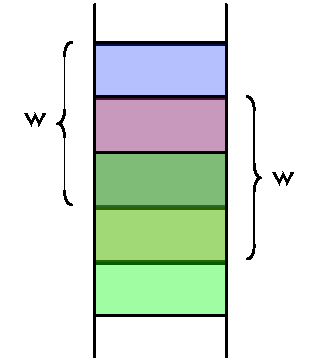
\includegraphics[scale=.6]{fig4/sorted-neighborhood.pdf}
    \end{column}
    \end{columns}
    
    % \begin{itemize}
    % \item Komplexität: % $O(n \cdot \log(n))$ oder $O(n \cdot w)$
    % \begin{itemize}
    % \item Schlüsselerzeugung: $O(n)$, Sortieren: $O(n \cdot \log(n))$;
    %   Vergleichen: $O( (n/w) \cdot (w^2)) = O(n \cdot w)$; 
    % Gesamt: $O(n \cdot \log(n))$ oder $O(n \cdot w)$
    % \end{itemize}
    % \end{itemize}
    
    \end{frame}
    
    %---------------------------------------------------------------------
    
    \begin{frame}
    \frametitle{Sortierte Nachbarschaft: Probleme}
    
    \begin{itemize}
    \item Genauigkeit schlecht
    \begin{itemize}
    \item Sortierkriterium bevorzugt immer Attribute
    \item Sind erste Buchstaben wichtiger für Identität als letzte?
    \item Ist Nachname wichtiger als Hausnummer?
    \end{itemize}
    \item Window vergrößern?
    \begin{itemize}
    \item Keine Hilfe
    \item Dominanz eines Attributes bleibt gleich, aber Laufzeit
      verschlechtert sich schnell 
    \end{itemize}
    \end{itemize}
    
    \end{frame}
    
    %---------------------------------------------------------------------
    
    
    \begin{frame}
    \frametitle{Multi-Pass-Technik}
    
    \begin{itemize}
    \item Sortieren und vergleichen nach mehreren Kriterien
    \item Kleinere Fenster
    \item Bildung der transitiven Hülle der Duplikate bis zu gegebener Länge
    \end{itemize}
    
    \begin{columns}[c]
    \begin{column}{6cm}
    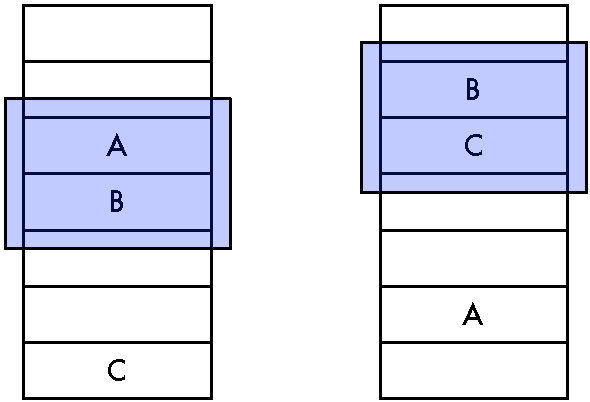
\includegraphics[scale=.6]{fig4/multi-pass.pdf}
    \end{column}
    \begin{column}{5cm}
    \begin{itemize}
    \item 1. Lauf: "`A matches B"'
    \item 2. Lauf: "`B matches C"'
    \item Transitivität: "`A matches C"'
    \end{itemize}
    \end{column}
    \end{columns}
    
    \end{frame}
    
    %---------------------------------------------------------------------
    
    
    \begin{frame}
    \frametitle{Vergleichsfunktionen}
    
    \begin{itemize}
    \item Vergleichsfunktionen für Felder (String $A$ und $B$), u.a.:
    \begin{itemize}
    \item \hl{Editierdistanz}: Anzahl der Editieroperationen (Einfügen,
      Löschen, Ändern) für Änderung von $A$ in $B$ 
    \item \hl{q-Grams}: Vergleich der Mengen aller Teilstrings von $A$ und $B$
      der Länge $q$ 
    \item \hl{Jaro-Distanz}: Berücksichtigung von gemeinsamen Zeichen
      (innerhalb der halben Stringlänge) und transponierten Zeichen (an
      anderer Position) 
    \item Jaccard, TFIDF, Soundex, ...
    \end{itemize}
    \end{itemize}
    
    \end{frame}
    %---------------------------------------------------------------------
    
    \begin{frame}
    \frametitle{Vergleichsfunktionen: Editierdistanz}
    
    \begin{itemize}
    \item \hl{Editierdistanz} (Levensthein-Distanz):
    \begin{itemize}
    \item Anzahl der Editieroperationen (Einfügen, Löschen, Ändern) für
      Änderung von $A$ in $B$  
    \item Beispiel:
    \hspace*{-1cm}\begin{sql}
    edit\_distance("Qualität", "Quantität") = 2 \\
    \1 $\Rightarrow$ update(3,'n') \\
    \1 $\Rightarrow$ insert(4,'t')
    \end{sql}
    \item Anwendung:
    \hspace*{-1cm}\begin{sql}
    \op{select} P1.Name, P2.Name \\
    \op{from} Produkt P1, Produkt P2 \\
    \op{where} edit\_distance(P1.Name, P2.Name) $<=$ 2
    \end{sql}
    \end{itemize}
    \end{itemize}
    
    \end{frame}
    
    %---------------------------------------------------------------------
    
    \begin{frame}
    \frametitle{Vergleichsfunktionen: q-Grams}
    
    \begin{itemize}
    \item \hl{q-Grams}: Menge aller Substrings der Länge $q$\\
    Qualität := \{ \_\_Q, \_Qu, Qua, ual, ali, lit, itä, tät, ät\_, t\_\_ \}
    \item Beobachtung: Strings mit kleiner Editierdistanz haben viele
      gemeinsame q-Grams, d.h. für Editierdistanz = $k$ mind.
    $$\max(|A|, |B|)-1-(k-1) \cdot q$$
     gemeinsame q-Grams
    
    \item \hl{Positionale q-Grams}: Ergänzung um Position im String \\
    Qualität := \{ (-1, \_\_Q), (0, \_Qu), (1, Qua), ... \}
    \begin{itemize}
    \item Filterung für effizienten Vergleich:
    \begin{itemize}
    \item COUNT: Anzahl der gemeinsamen q-Grams
    \item POSITION: Positionsunterschied zwischen korrespondierenden
      q-Grams $\leq$ k 
    \item LENGTH: Differenz der Stringlängen $\leq$ k
    \end{itemize}
    \end{itemize}
    \end{itemize}
    
    \end{frame}
    
    %---------------------------------------------------------------------
    
    \begin{frame}
    \frametitle{Domänenspezifische Vergleichsfunktionen}
    
    \begin{itemize}
    \item Vergleiche in Feldern mit spezieller Bedeutung (Namen, Codes,
      Adressen)
    \begin{itemize}
    \item Soundex: phonetische Kodierung, speziell für ähnlich klingende
      Namen ("Hilbert" = "Heilbpr") 
    \item Ausnutzung von Codes (TXL = Berlin-Tegel)
    \item Namenskonventionen
    \begin{itemize}
    \item Hawking, Stephen = Stephen Hawking
    \item Hauptstr. = Hauptstraße
    \end{itemize}
    \end{itemize}
    \end{itemize}
    
    \end{frame}
    
    %---------------------------------------------------------------------
    %
    %\begin{frame}
    %\frametitle{Vergleich von Records}
    %
    %\begin{itemize}
    %\item Basierend auf �hnlichkeit der Felder
    %\item Problem:
    %\begin{itemize}
    %\item Feldanzahl und Art k�nnen sich unterscheiden
    %\item Auswahl relevanter Felder
    %\item Wichtung der Felder
    %\begin{itemize}
    %\item 8 Pkt. f�r �bereinstimmung Nachname
    %\item 6 Pkt. f�r f�r �bereinstimmung Vorname
    %\item 4 Pkt. f�r f�r �bereinstimmung Geburtstag
    %\item 1 Pkt. f�r f�r �bereinstimmung Geschlecht
    %\item Gesamt �ber 11 Pkt. $\rightarrow$ Treffer
    %\end{itemize}
    %\end{itemize}
    %\item Ans�tze
    %\begin{itemize}
    %\item Probabilistische Verfahren 
    %\item Nicht-Probabilistische Verfahren
    %\end{itemize}
    %\end{itemize}
    %
    %\end{frame}
    %
    %%---------------------------------------------------------------------
    %
    %\begin{frame}
    %\frametitle{Probabilistische Verfahren}
    %
    %\begin{center}
    %\includegraphics[scale=.6]{fig3/prob-linkage.pdf}
    %\end{center}
    %
    %\end{frame}
    %
    %%---------------------------------------------------------------------
    %
    %\begin{frame}
    %\frametitle{Probabilistische Verfahren /2}
    %
    %\begin{itemize}
    %\item Vergleichsvektor enth�lt "`Features"' $\gamma(R.A_i,S.A_i)$
    %\begin{itemize}
    %\item z.B. "`Nachnamen sind gleich"'
    %\end{itemize}
    %$$
    %\gamma = (\gamma^1(t_R.A_1,t_S.A_1), \gamma^2(t_R.A_2,t_S.A_2), \dots,
    %\gamma^k(t_R.A_k,t_S.A_k))$$
    % 
    %\item Wahrscheinlichkeiten
    %\begin{itemize}
    %\item $m(\gamma) = P(\gamma | (t_R, t_S) \in M)$ f�r Match
    %\item $u(\gamma) = P(\gamma | (t_R, t_S) \in U)$ f�r Non-Match
    %\item Ableitung von $m(\gamma)$ und $u(\gamma)$ z.B. durch
    %  Voruntersuchung (z.B. EM-Algorithmus (Expectation-Maximization-Algorithmus))
    %\end{itemize}
    %\item Ablauf
    %\begin{enumerate}
    %\item Bestimmung der Einzelgewichte f�r Attribute
    %\item Berechnung des Gesamt-Scores
    %\item Entscheidung �ber Match (M) bzw. Non-Match (U)
    %\end{enumerate}
    %\end{itemize}
    %
    %\end{frame}
    %
    %%---------------------------------------------------------------------
    %
    %\begin{frame}
    %\frametitle{Nicht-Probabilistische Verfahren (Deterministische Verfahren)}
    %
    %\begin{itemize}
    %\item Wissensbasierte Verfahren
    %\begin{itemize}
    %\item Funktionale Abh�ngigkeiten auf Instanzebene
    %\item Matching-Regeln
    %\end{itemize}
    %\item Data-Mining-Verfahren
    %\begin{itemize}
    %\item Clustering
    %\item Entscheidungsbaumverfahren
    %\end{itemize}
    %\item Distanzbasierte Verfahren
    %\end{itemize}
    %
    %\end{frame}
    %
    %%---------------------------------------------------------------------
    %
    %\begin{frame}
    %\frametitle{Regelbasiertes Matching}
    %
    %\begin{itemize}
    %\item IntelliClean [Lee et al. 2000]
    %\item Nutzung von Dom�nenwissen durch deklarative Regeln
    %\hspace*{-1cm}\begin{sql}
    %\op{if} A.Name = B.Name \\
    %\op{and} field\_similarity (A.Adresse, B.Adresse) \\
    %\op{then} \dots 
    %\end{sql}
    %\item Regeltypen
    %\begin{itemize}
    %\item Duplicate identification rules: Bedingungen f�r �bereinstimmung
    %  mit Sicherheitsfaktor 
    %\item Merge/purge rules: Aktionen zum Verschmelzen
    %\item Update rules: Manipulation von Feldern (z.B. bei leeren Feldern)
    %\item Alert rules: Benachrichtigung bei notwendigem Review
    %\end{itemize}
    %\item Regelauswertung durch Inferenz-Engine
    %\end{itemize}
    %
    %\end{frame}
    %---------------------------------------------------------------------
    
    \begin{frame}
    \frametitle{Datenkonflikte}
    
    \begin{itemize}
    \item Datenkonflikt: Zwei Duplikate haben unterschiedliche
      Attributwerte für semantisch gleiches Attribut
    \begin{itemize}
    \item im Gegensatz zu Konflikten mit Integritätsbedingungen
    \item Bsp.: Amazon\\
    \begin{tabular}{|l|l|l|c|}
    \hline
    0766607194 & H. Melville & & 3.99 \\
    \hline
    0766607194 & Herman Melville &  Moby Dick & 5.99 \\
    \hline
    \end{tabular}
    
    \end{itemize}
    
    \item Datenkonflikte entstehen 
    \begin{itemize}
    \item innerhalb eines Informationssystems (intra-source) und
    \item bei der Integration mehrerer Informationssysteme (inter-source)
    \end{itemize}
    \item Voraussetzung: Duplikat, d.h. Identität schon festgestellt
    \item erfordert: Konfliktauflösung (Purging, Reconciliation)
    \end{itemize}
    
    \end{frame}
    
    %---------------------------------------------------------------------
    
    
    \begin{frame}
    \frametitle{Datenkonflikte: Entstehung}
    
    \begin{itemize}
    \item Mangels Integritätsbedingungen oder Konsistenz-Checks
    \item Bei redundanten Schemata
    \item Bei Entstehung von Duplikaten
    \item Nicht korrekte Einträge
    \begin{itemize}
    \item Tippfehler, Übertragungsfehler
    \item Falsche Rechenergebnisse
    \end{itemize}
    \item obsolete Einträge
    \begin{itemize}
    \item div. Aktualisierungszeitpunkte
    \begin{itemize}
    \item ausreichende Aktualität einer Quelle
    \item verzögerte Aktualisierung
    \end{itemize}
    \item vergessene Aktualisierung
    \end{itemize}
    \end{itemize}
    
    
    \end{frame}
    
    
    %---------------------------------------------------------------------
    
    \begin{frame}
    \frametitle{Datenkonflikte: Behebung}
    
    \begin{itemize}
    \item Referenztabellen für exakte Wertabbildung
    \begin{itemize}
    \item Z.B. Städte, Länder, Produktnamen, Codes...
    \end{itemize}
    \item Ähnlichkeitsmaße
    \begin{itemize}
    \item bei Tippfehlern, Sprachvarianten (Meier, Mayer,...)
    \end{itemize}
    \item Standardisieren und Transformieren
    \item Nutzung von Hintergrundwissen (Metadaten)
    \begin{itemize}
    \item bzgl. Konventionen (landestypische Schreibweisen)
    \item Ontologien, Thesauri, Wörterbücher zur Behandlung von Homonymen,
      Synonymen, \dots
    \end{itemize}
    \item Bei der Integration
    \begin{itemize}
    \item Präferenzordnung über Datenquellen nach Aktualität, Trust
      (Vertrauen) usw. 
    \item Konfliktlösungsfunktionen
    \end{itemize}
    \end{itemize}
    
    \end{frame}
    
    
    %---------------------------------------------------------------------
    
    \begin{frame}
    \frametitle{Record Linkage mit Python Record Linkage Toolkit}
    
    \begin{itemize}
    \item Python-Framework für Record Linkage-Aufgaben
    \item Komponenten
    \begin{itemize}
    \item Indexer: Komponente zur Gruppierung von Kandidaten, z.B. Blocking und Sortierte Nachbarschaft
    \item Vergleichs- und Ähnlichkeitsfunktionen
    \item Klassifikatoren für Einteilung in Matches / Non-Matches
    \item Datensätze
    \end{itemize}
    \item nutzbar mit Pandas 
    \end{itemize}
    
    \end{frame}
    
    %---------------------------------------------------------------------
    
    \begin{frame}[shrink]
    \frametitle{Python Record Linkage Toolkit}
    
    \begin{python}
    \pycomment{Daten laden} \\
    from recordlinkage.datasets import load\_febrl1 \\
    data = load\_febrl1() \\
    \pycomment{Blocking als Indexer nutzen} \\
    indexer = recordlinkage.Index() \\
    indexer.block('given\_name') \\
    \pycomment{Kandidaten für Vergleiche} \\
    candidates = indexer.index(data) \\
    \\
    \pycomment{Vergleichsfunktion} \\
    cmp = recordlinkage.Compare() \\
    cmp.exact('given\_name', 'given\_name', label='given\_name') \\
    cmp.string('surname', 'surname', method='jarowinkler', \\
    \1 threshold=0.85, label='surname') \\
    ...\\
    features = cmp.compute(candidates, data) 
    \end{python}
    
    \end{frame}
    
    %---------------------------------------------------------------------
    \begin{frame}
    \frametitle{Python Record Linkage Toolkit: Matching}
    
    \begin{itemize}
    \item DataFrame \texttt{features} enthält alle Record-Paare und die Features
    \item Summieren der Werte pro Zeile (\texttt{axis=1})
    \end{itemize}
    \begin{python}
    features.sum(axis=1).value\_counts().\textbackslash \\
    \1 sort\_index(ascending=False)
    \end{python}
    
    \begin{itemize}
    \item Auswahl über Schwellwert
    \end{itemize}
    
    \begin{python}
    matches = features[features.sum(axis=1) > 3]
    \end{python}
    
    \end{frame}
    %---------------------------------------------------------------------
    
    \section{Datenreduktion}
    
    \begin{frame}
    \frametitle{Datenreduktion}
    
    
    \begin{itemize}
    \item \hl{Ziel:} Reduzierung der Daten
    \begin{itemize}
    \item kleinere Datenmenge $\leadsto$ schnellere Verarbeitung: \hl{Sampling}
    \item Eliminierung irrelevanter Daten: \hl{Dimensionsreduktion} z.B. durch Hauptkomponentenanalyse (PCA)
    \item Erhöhung des Abstrationslevels: \hl{Aggregation}, \hl{Diskretisierung}
    \end{itemize}
    \item Erhaltung der Konsistenz der Daten
    \end{itemize}
    \end{frame}
    
    %---------------------------------------------------------------------
    
    \begin{frame}
    \frametitle{Sampling}
    
    \begin{itemize}
    \item Idee: kleine, zufällig gewählte, uniforme Stichprobe $S$ stellt gute
      Repräsentation der Daten (Grundgesamtheit) dar
    \begin{itemize}
    \item Datenreduktion
    \item Erzeugung eines Testdatensatzes zur Validierung
    \item approximiertes Anfrageergebnis: Ausführung einer modifizierten
      Anfrage auf $S$
    \end{itemize}
    \item Beispiel:
    
    {\small
    \begin{tabular}{ccccccccccccccc}
    3 & \fbox{4} & 7 & \fbox{8} & 6 & 1 & \fbox{2} & 5 & \fbox{9} & 6 & 2
    & \fbox{7} & 4 & 6 & \fbox{1}
    \end{tabular}}
    \vspace*{.5em}
    
    \hspace*{-.5cm}\begin{algo}
    \op{select} \emph{aggr} \op{from} Data \op{where} item > 5
    \end{algo}
    \begin{itemize}
    \item \emph{aggr} = \texttt{avg} $\leadsto$ 8 (exakt: 7)
    \item \emph{aggr} = \texttt{count} für $\frac{3}{6}$ $\leadsto$ 7.5 (exakt: 7)
    \end{itemize}
    \end{itemize}
    \end{frame}
    
    %---------------------------------------------------------------------
    
    \begin{frame}
    \frametitle{Sampling: Verfahren}
    
    \begin{itemize}
    \item \hl{einfaches randomisiertes Sampling:} jedes Element der Grundgesamtheit ist mit der gleichen Wahrscheinlichkeit in der Stichprobe enthalten
    \item \hl{stratifiziertes ("`geschichtetes") Sampling:} 
    \begin{itemize}
    \item Aufteilung der Grundgesamtheit in Gruppen (Strata, Schichten)
    \item Festlegung der Stichprobengröße pro Schicht
    \item Sampling pro Schicht
    \item \hl{erfordert Vorabkenntnis der Schichtungsmerkmale}, z.B. Bevölkerungsgruppen bei Wahlen
    \end{itemize}
    \item \hl{Cluster Sampling:} Clustering der Daten, zufallsbasierte Auswahl der Cluster, alle Elemente der gewählten Cluster bilden Stichprobe $\leadsto$ Reduzierung des Erhebungsaufwandes (Befragung etc.)
    \end{itemize}
    \end{frame}
    
    %---------------------------------------------------------------------
    
    \begin{frame}
    \frametitle{Reservoir-Sampling}
    
    [Vitter 85]
    \begin{itemize}
    \item Ziel: Verwaltung einer zufälligen Stichprobe konstanter Größe
      für Grundgesamtheit \textbf{unbekannter Größe} (z.B. Datenstrom)
    \end{itemize}
    
    \begin{center}
    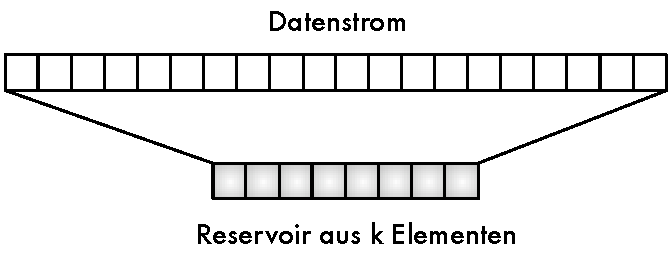
\includegraphics[scale=.7]{fig4/reservoir-sampling.pdf}
    \end{center}
    
    \end{frame}
    
    %---------------------------------------------------------------------
    
    \begin{frame}
    \frametitle{Reservoir-Sampling /2}
    
    \begin{itemize}
    \item Prinzip
    \begin{itemize}
    \item Übernahme der ersten $k$ Elemente des Stroms in das Reservoir
      $S$
    \item Ankunft des $i$-ten Elementes
    \begin{itemize}
    \item zum Reservoir $S$ hinzufügen mit Wahrscheinlichkeit
      $\frac{k}{i}$
    \item falls hinzugefügt: zufällig ausgewähltes Element aus $S$ löschen
    \item Test nicht für jedes Element, sondern Anzahl der zu
      überspringenden Elemente im voraus bestimmen
    \end{itemize}
    \end{itemize}
    \end{itemize}
    
    \end{frame}
    
    %---------------------------------------------------------------------
    
    \begin{frame}
    \frametitle{Sampling in Pandas}
    
    \begin{itemize}
    \item Einfaches Sampling eines DataFrames
    \end{itemize}
    \begin{python}
    df.sample(n=10)
    \end{python}
    
    \begin{itemize}
    \item Sampling mit reproduzierbaren Ergebnissen
    \end{itemize}
    \begin{python}
    df.sample(n=10, random\_state=42)
    \end{python}
    
    \begin{itemize}
    \item Sampling mit prozentualer Größe
    \end{itemize}
    
    \begin{python}
    df.sample(frac=0.25, random\_state=42)
    \end{python}
    
    \end{frame}
    
    %---------------------------------------------------------------------
    
    \begin{frame}
    \frametitle{Sampling in Pandas /2}
    
    \begin{itemize}
    \item Aufteilung in Trainings- und Testdaten muss überlappungsfrei sein
    \end{itemize}
    
    \begin{python}
    from sklearn.model\_selection import train\_test\_split \\
    train\_data, test\_data = train\_test\_split(df, \\
    \1 test\_size=0.2, random\_state=42)
    \end{python}
    \end{frame}
    %---------------------------------------------------------------------
    
    \begin{frame}
    \frametitle{Zusammenfassung}
    
    \begin{itemize}
    \item Wiederholung: Statistik und Daten
    \item Daten
    \begin{itemize}
    \item Arten \& Eigenschaften
    \item Datenqualität
    \end{itemize}
    \item Datenbereinigung
    \begin{itemize}
    \item als Teil des Data-Science-Prozesses
    \item wichtige Teilaufgaben: Profiling, fehlende Werte, Ausreißer,
      Record Linkage
    \end{itemize}
    \item Literatur: 
    \begin{itemize}
    \item Ester, Sander: "`Knowledge Discovery in Databases"',
      Springer-Verlag, 2000
    \item Fahrmeir, Künstler, Pigeot, Tutz: "`Statistik -- Der Weg zur
      Datenanalyse"', Springer-Verlag  
    \item Batini, Scannapieco: "`Data Quality: Concepts, Methodologies and
      Techniques"', Springer-Verlag
    \end{itemize}
    \end{itemize}
    
    \end{frame}
    